\documentclass[10pt]{beamer}

\usetheme{metropolis}
\usepackage{appendixnumberbeamer}

\usepackage{booktabs}
\usepackage[scale=2]{ccicons}
\usepackage{graphicx}
\usepackage{hyperref}
\usepackage{circuitikz}
\usepackage{pdflscape}
\usepackage{smartdiagram}

\usepackage{color}
\usepackage{listings}

\lstset{
	basicstyle=\footnotesize\ttfamily,
    keepspaces=true,
    showstringspaces=false,
    language=PHP,
    commentstyle=\ttfamily,
}

\usepackage[OT4]{polski}
\usepackage[utf8]{inputenc}

\usepackage{pgfplots}
\usepgfplotslibrary{dateplot}

\usepackage{xspace}
\newcommand{\themename}{\textbf{\textsc{metropolis}}\xspace}

\setbeamertemplate{frame footer}{}
\setbeamertemplate{frame numbering}{}

\usetikzlibrary{shapes,arrows}

\tikzstyle{decision} = [diamond, draw, fill=blue!20, 
    text width=4.5em, text badly centered, node distance=3cm, inner sep=0pt]
\tikzstyle{block} = [rectangle, draw, fill=blue!20, 
    text width=5em, text centered, rounded corners, minimum height=4em]
\tikzstyle{line} = [draw, -latex']
\tikzstyle{cloud} = [draw, ellipse,fill=red!20, node distance=3cm,
    minimum height=2em]


\title{Wprowadzenie do systemów internetowych}

\subtitle{Projektowanie i programowanie systemów internetowych I}
\author{mgr inż. Krzysztof Rewak}
\date{\today}
\institute{Wydział Nauk Technicznych i Ekonomicznych \\ Państwowa Wyższa Szkoła Zawodowa im. Witelona w Legnicy}

\begin{document}

\maketitle

\begin{frame}{Plan prezentacji}
  \setbeamertemplate{section in toc}[sections numbered]
  \tableofcontents[hideallsubsections]
\end{frame}


\section{Ramowy plan semestru}

\begin{frame}{Planowany rozkład jazdy: luty - kwiecień}
	Wykład 1: Wprowadzenie do systemów internetowych
	
	Wykład 2: Statyczne strony w internecie, technologie HTML + CSS
	
	Wykład 3: Narzędzia deweloperskie
	
	Wykład 4: Obsługiwanie zapytań, protokół HTTP
	
	Wykład 5: Wzorzec architektoniczny MVC
	
	Wykład 6: Środowisko deweloperskie
	
	Wykład 7: Implementacja logiki biznesowej
\end{frame}

\begin{frame}{Planowany rozkład jazdy: kwiecień - czerwiec}
	Wykład 8: Internetowe bazy danych
	
	Wykład 9: Mapowanie relacyjno-obiektowe
	
	Wykład 10: Uwierzytelnianie i autoryzacja użytkowników
	
	Wykład 11: Asynchroniczne interakcje z serwerem
	
	Wykład 12: Mechanizmy pamięci podręcznej i optymalizacja
	
	Wykład 13: RWD, SEO i inne skrótowce
	
	Wykład 14: Rozszerzanie systemów internetowych
	
	Wykład 15: Kolokwium zaliczeniowe - tzw. \emph{zerówka}
\end{frame}

\section{Warunki zaliczenia kursu}

\begin{frame}{Formy zajęć}
	\begin{figure}
		\resizebox{.5\linewidth}{!}{W + P}
	\end{figure}
	
	\ \\
	
	\textbf{wykład} - teoretyczna część kursu; przedstawienie najważniejszych zagadnień związanych z aplikacjami webowymi, pokazanie metodologii pracy, przestawienie współczesnych narzędzi do tworzenia systemów internetowych
	
	\textbf{projekt} - praktyczna część kursu; praca zespołowa nad projektowaniem, implementacją oraz wdrożeniem konkretnego systememu internetowego
\end{frame}

\begin{frame}{Warunki zaliczenia wykładu}
	Wykład kończy się egzaminem podsumowującym wiedzę przyswojoną w trakcie semestru. Egzamin - w zależności od liczby przystępujących osób - odbędzie się w formie pisemnej lub ustnej.
	
	Student, który otrzyma z projektu ocenę niedostateczną nie może podchodzić do egzaminu.
\end{frame}

\begin{frame}{Warunki zaliczenia wykładu}	
	Ponadto na wykładach:
	\begin{itemize}
		\item będzie sprawdzana lista obecności na zasadzie białej listy;
		\item będzie mierzona (pozytywna i negatywna) aktywność studentów.
	\end{itemize}
	
	Zachęcam do uczęszczania na wykłady.
\end{frame}

\begin{frame}{Ocena końcowa}
	\begin{figure}
		\resizebox{.66\linewidth}{!}{0.3W + 0.7L}
	\end{figure}
	
	Ocena niedostateczna z jednej formy rzutuje na ocenę niedostateczną za całość!
	
	Przykładowo:
	\begin{itemize}
		\item 3.0 E + 5.0 L = 4.4 $\Rightarrow$ \textbf{4.5}
		\item 4.5 E + 4.0 L = 4.15 $\Rightarrow$ \textbf{4.0}
		\item 2.0 E + 5.0 L = 4.1 $\Rightarrow$ \textbf{2.0}
	\end{itemize}
\end{frame}

\begin{frame}{Bonusy}	
	Osoby, które otrzymały ocenę z projektu \textbf{$p = 5.0$}, zostaną zwolnione z egzaminu z przepisaną oceną.
\end{frame}

\begin{frame}{Bonusy}	
	Wysoka frekwencja oraz aktywność na wykładach mogą rzutować na obniżenie progu przepisywanej oceny do $p \geq 4.5$ dla indywidualnych studentów.
\end{frame}

\begin{frame}{Bonusy}		
	W trakcie semestru organizowane będą dodatkowe zwolnienia z egzaminu w formie interaktywnych \emph{kartkówek} z bieżącego materiału.
	
	Student, który otrzyma najwięcej punktów z danej \emph{kartkówki}, zostanie zwolniony z egzaminu z przepisaną oceną z projektu.
\end{frame}

\section{Wprowadzenie do systemów internetowych}

\begin{frame}[fragile]{Czym są systemy internetowe?}
	Systemem internetowym można nazwać program komputerowy umieszczony i uruchomiony na serwerze. Jest dostępny przez sieć Internet przez konkretny adres IP i port lub domenę. 
	
	Nie należy utożsamiać systemów internetowych z stronami internetowymi, ponieważ te drugie są jedynie częścią ogromu zastosowań pierwszych.
\end{frame}

\begin{frame}[fragile]{Budowa klasycznego systemu internetowego}
	\begin{tikzpicture}[node distance=3cm, minimum size=2cm, auto]
	
		\node [block] (core) {jądro systemu};
	
		\node [block, above of=core] (server) {funkcje serwerowe};
		\node [block, left of=core] (database) {bazy danych};
		\node [block,above left of=core] (cache) {serwery cache};
		\node [block, below left of=core] (filesystem) {systemy plików};
		\node [block, below of=core] (services) {inne serwisy};
	
		\path [line] (core) -- node {} (server);
		\path [line] (server) -- node {} (core);
	
		\path [line] (core) -- node {} (database);
		\path [line] (database) -- node {} (core);
	
		\path [line] (core) -- node {} (cache);
		\path [line] (cache) -- node {} (core);
	
		\path [line] (core) -- node {} (filesystem);
		\path [line] (filesystem) -- node {} (core);
	
		\path [line] (core) -- node {} (services);
		\path [line] (services) -- node {} (core);
		
		\node [circle, fill=orange,inner sep=3pt, right of=core] (http) {serwer HTTP};
	
		\path [line] (http) -- node {} (core);
		\path [line] (core) -- node {} (http);
		
		\node [block, above right of=http] (browser) {przeglądarka};
		\node [block, below right of=http] (api) {inna aplikacja};
	
		\path [line] (http) -- node {} (browser);
		\path [line] (browser) -- node {} (http);
	
		\path [line] (http) -- node {} (api);
		\path [line] (api) -- node {} (http);
	
	\end{tikzpicture}
\end{frame}

\begin{frame}[fragile]{Systematyka: podmiot wykonujący}
	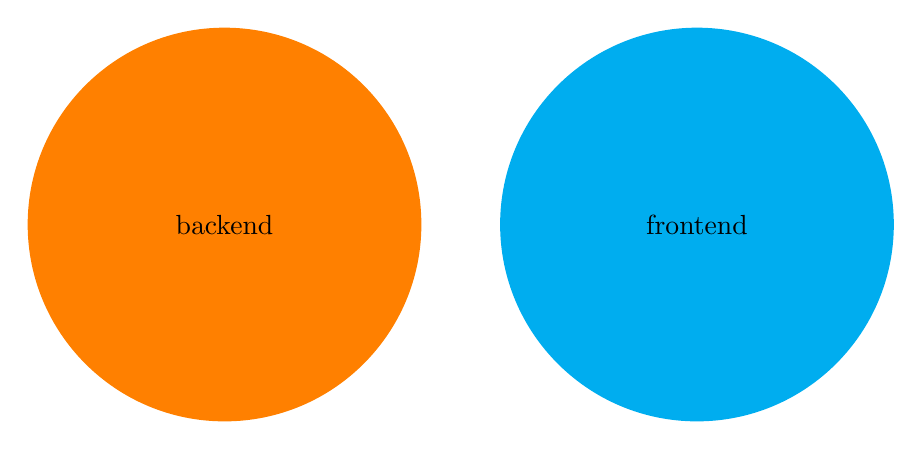
\begin{tikzpicture}[node distance=3cm, minimum size=5cm, auto]
		
		\node [circle, fill=orange,inner sep=5pt] (backend) {backend};
		
		\node [circle,inner sep=3pt, right of=backend] (x) {};
		
		\node [circle, fill=cyan,inner sep=5pt, right of=x] (frontend) {frontend};
	
	\end{tikzpicture}
\end{frame}


\begin{frame}[fragile]{Systematyka: przeznaczneie}
	Można między innymi wyróżnić następujące typy systemów internetowych:
	\begin{itemize}
		\item systemy zarządzania treścią
		\item systemy e-commerce
		\item systemy CRM i  ERP
		\item systemy mapujące dane
		\item systemy wystawiające API
		\item systemy bankowe
		\item platformy społecznościowe
	\end{itemize}
\end{frame}

\begin{frame}[fragile]{Języki programowania backendu}
	\begin{itemize}
		\item PHP (83\% z $10^7$ najpopularniejszych stron internetu, Facebook, Wikipedia, Yahoo, Wordpress)
		\item Python (YouTube)
		\item Ruby (Twitter)
		\item C\# (Bing, strony Microsoftu)
		\item Java (Amazon, Linkedin)
		\item JavaScript (eBay)
	\end{itemize}
	
	Podane przykłady to w niektórych przypadkach uproszczenia. Przykładowo Facebook jest zbudowany z łączących się ze sobą serwisów napisanych w PHP, Pythonie, C++, Javie, Erlangu, D, Haskellu i kilku innych, jednak jądro budowane jest w PHP.
\end{frame}

\begin{frame}[fragile]{Wynajdywanie koła na nowo}
	Każdy język posiada własne zestawy narzędzi, tzw. frameworki, które ułatwiają programowanie. Oto najpopularniejsze web-frameworki na obecną chwilę:
	\begin{itemize}
		\item Symfony, Laravel, Zend, Phalcon, Yii
		\item Django, Flask
		\item Ruby on Rails
		\item ASP.NET MVC, ASP.NET Core
		\item Spring
		\item Node.js, Angular, React, Vue.js
	\end{itemize}
\end{frame}

\section{Podsumowanie}

\begin{frame}{Bibliografia i ciekawe źródła}
  
	\begin{thebibliography}{9}
	
		\bibitem{rewak}
		Krzysztof Rewak,
		\textit{Projektowanie i programowanie obiektowe},
		materiały do zajęć laboratoryjnych
	
	\end{thebibliography}

\end{frame}

\appendix

\begin{frame}[standout]
	Pytania?
\end{frame}

\begin{frame}{}

	Kod prezentacji dostępny jest w repozytorium git pod adresem \texttt{https://bitbucket.org/krewak/pwsz-ppsi} \\ \ \\

	\begin{figure}
		\centering
		\href{https://bitbucket.org/krewak/pwsz-ppsi}{
			
\includegraphics[width=.15\textwidth]{../_template/bitbucket.png}
		}
	\end{figure}
	
	Wszystkie informacje dot. kursu dostępne są pod adresem \texttt{http://pwsz.rewak.pl/kursy/4} \\ \ \\

	\begin{figure}
		\centering
		\href{http://pwsz.rewak.pl/kursy/3}{
			
\includegraphics[width=.15\textwidth]{../_template/rewak.png}
		}
	\end{figure}

\end{frame}

\end{document}
